\documentclass[conference]{IEEEtran}
\IEEEoverridecommandlockouts
\usepackage{cite}
\usepackage{amsmath,amssymb,amsfonts}
\usepackage{algorithmic}
\usepackage{graphicx}
\usepackage{textcomp}
\usepackage{xcolor}
\usepackage{booktabs}
\usepackage{multirow}
\usepackage{subcaption}
\def\BibTeX{{\rm B\kern-.05em{\sc i\kern-.025em b}\kern-.08em
    T\kern-.1667em\lower.7ex\hbox{E}\kern-.125emX}}

\begin{document}

\title{Text-as-Image Compression for Vision-Language Models: How Far Can Rendered Text Replace Text Tokens in Long-Context Retrieval?}

\author{\IEEEauthorblockN{1\textsuperscript{st} Ahnaf Tahmid}
\IEEEauthorblockA{\textit{Dept. of CSE} \\
\textit{United International University}\\
Dhaka, Bangladesh \\
mtahmid2310203@bscse.uiu.ac.bd}
\and
\IEEEauthorblockN{2\textsuperscript{nd} Quazi Nazib Zaman}
\IEEEauthorblockA{\textit{Dept. of CSE} \\
\textit{United International University}\\
Dhaka, Bangladesh \\
qzaman2320230@bscse.uiu.ac.bd}
\and
\IEEEauthorblockN{3\textsuperscript{rd} Fouzia Jahan Dhola}
\IEEEauthorblockA{\textit{Dept. of CSE} \\
\textit{United International University}\\
Dhaka, Bangladesh \\
fdhola2320182@bscse.uiu.ac.bd}
}

\maketitle

\begin{abstract}
Large language models (LLMs) are now used on long documents, but every extra text token makes the prompt longer and the computation heavier. Vision-language models can read text from pictures, so there is another option: turn the document into an image and let the vision encoder describe it with a small number of visual tokens. We still do not know when this ``text-as-image'' idea stops working, or whether the saved tokens really make the model faster. In this paper, we test the open vision-language model Gemma~4 (31B) on a needle-in-a-haystack retrieval task based on RULER. We build a simple pipeline that cleans the text and draws it onto an image. We use synthetic documents of 500, 1{,}000, and 1{,}500 tokens and five canvas settings (named after 70 to 1{,}120 visual tokens), and we compare the results with plain text input. We keep the model, the question, and the decoding (temperature $0$) the same, so only the input type changes. Image input cuts the prompt by 53.5\%, 72.9\%, and 82.3\% (compression ratios of about $2.2\times$, $3.7\times$, and $5.7\times$) for the three lengths. Retrieval accuracy is 100\%, 80\%, and 20\%, while plain text stays at 100\%. The mistakes come from reading the image (wrong or missing characters), not from reasoning, and the image path was slower than text in 13 of 15 runs. Regression analysis reveals that text-as-image achieves net token savings only beyond a break-even threshold of $\approx 181$ words ($\mathrm{CR} > 1.0$), identifying an optimal operating sweet spot between 397 and 434 words where $\ge 50\%$ prompt token savings are achieved with 100\% retrieval accuracy before OCR degradation emerges. These early results show the trade-off between compression and accuracy, and they give a reusable pipeline for larger studies.
\end{abstract}

\begin{IEEEkeywords}
optical context compression, text-as-image, vision-language models, long-context retrieval, needle-in-a-haystack, visual tokens, Gemma~4
\end{IEEEkeywords}

\section{Introduction}
Many applications today need language models to read long inputs, such as document analysis, retrieval-augmented generation, and agents. The problem is that each extra text token adds memory use, delay, and cost, and attention grows quadratically with the sequence length \cite{vaswani2017attention}. Vision-language models (VLMs) give us another way to feed in data. A vision encoder turns an image into a short list of visual tokens \cite{dosovitskiy2021vit}. A page full of text can be drawn as one image, so the same content may need far fewer tokens. This idea is called \emph{optical context compression} \cite{wei2025deepseekocr,cheng2025glyph}, and it is close to language modeling with pixels \cite{rust2023pixel}.

Still, several questions are open. Most earlier work builds special encoders or trains new models. It is less clear what happens when we take a general VLM as it is and just show it the context as an image. We do not know at which compression ratio retrieval starts to fail, whether the image resolution matters, or whether fewer tokens give a real speed gain in a normal serving setup. Long-context benchmarks like RULER \cite{hsieh2024ruler} and BABILong \cite{kuratov2024babilong} use text inputs only, so they do not test this change of input type.

We study these questions with Gemma~4 (\texttt{gemma4:31b}) running through Ollama. We build a controlled text-as-image pipeline and test it on a synthetic needle-in-a-haystack task, using three context lengths and five rendering settings. Four research questions guide the work:
\begin{itemize}
\item \textbf{RQ1} (Compression): how well can text be compressed into visual tokens without losing accuracy?
\item \textbf{RQ2} (Model comparison): how does this differ between models (Gemma~4 and Qwen3.5)?
\item \textbf{RQ3} (Degradation point): at what compression ratio does performance drop?
\item \textbf{RQ4} (Speed): do fewer tokens mean lower latency?
\end{itemize}
This paper answers RQ1, RQ3, and RQ4 for Gemma~4. RQ2 and the other tasks in our full plan (summarization on CNN/DailyMail and reasoning on BABILong) are left for future work.

Our contributions are:
\begin{enumerate}
\item A reproducible pipeline that cleans, wraps, and draws any text onto an image with five canvas settings, plus a RULER-style generator where we control the position of the needle.
\item A full grid test ($3$ context lengths $\times$ $5$ settings) of Gemma~4, comparing text input (Condition~A) with image input (Condition~B) in accuracy, token count, compression ratio, and latency.
\item A look at how accuracy drops. The errors come from reading the image, and they appear once the context gets longer than about 1{,}000 tokens at a fixed canvas width. We also report honestly that the nominal token budgets did not change the real token count in our setup.
\item A quantitative threshold and operating zone analysis establishing the break-even boundary ($\approx 181$ words), the $2\times$ compression sweet spot ($397$--$434$ words), and the empirical degradation cliff, providing concrete decision rules for optical context compression.
\end{enumerate}

Our method works for any text that can be drawn clearly on an image and any model that accepts images. However, our data is synthetic English text of up to 1{,}500 tokens, so we cannot yet say the same holds for real documents or longer contexts.

The rest of the paper is organized as follows. Section~\ref{sec:related} covers related work, Section~\ref{sec:method} explains the method, Section~\ref{sec:setup} gives the experimental setup, Section~\ref{sec:results} shows the results, Section~\ref{sec:discussion} discusses limitations, and Section~\ref{sec:conclusion} concludes.

\section{Related Work}
\label{sec:related}
\textbf{Long-context evaluation.} A common way to test long-context ability is the needle-in-a-haystack test. RULER extends it to several tasks with growing sequence length \cite{hsieh2024ruler}. Other work shows that models use information differently depending on where it sits in the context \cite{liu2024lost}, and BABILong adds multi-hop reasoning over very long inputs \cite{kuratov2024babilong}. All of these use text input, so none of them checks what happens when the input type changes.

\textbf{Visual representation of text.} Language modeling with pixels removes the tokenizer and draws the text as images \cite{rust2023pixel}. More recently, DeepSeek-OCR studies optical context compression with its own vision encoder. It reports good text recovery at moderate compression and a drop when compression grows \cite{wei2025deepseekocr}. Glyph draws long text as images and trains a vision-language model to read them, which makes the effective context window larger \cite{cheng2025glyph}.

\textbf{Gap.} These methods train or adapt the model for the task. What is missing is a careful test of a general, openly available VLM that gets rendered text without any extra training, with clear token counts and latency numbers. Our work tries to fill this gap.

\section{Methodology}
\label{sec:method}

\subsection{Experimental Conditions}
We define three conditions to isolate the effect of using visual tokens. In \textbf{Condition A} (baseline), the input is text only, and the model gives an answer. In \textbf{Condition B} (main), the context is drawn as an image and sent with the question. In \textbf{Condition C} (hybrid), part of the text is kept and the rest is sent as an image, together with the question. We only run Conditions~A and~B in this paper.

\subsection{Text-to-Image Pipeline}
The pipeline has three steps. (i) \emph{Normalization}: we apply Unicode NFKC, fix the line endings, and merge repeated spaces. (ii) \emph{Layout}: we wrap paragraphs at a fixed number of characters and leave a blank line between paragraphs. (iii) \emph{Rasterization}: we draw the lines in black Arial text on a white RGB canvas. The canvas height depends on the number of lines, and we save the result as a PNG file. The five canvas settings are listed in Table~\ref{tab:configs}. They are named after the visual-token budgets $k\in\{70,140,280,560,1120\}$ from our proposal. A larger budget gives a wider canvas, a bigger font, and more line spacing. Fig.~\ref{fig:render} shows two examples.

\begin{table}[t]
\caption{Canvas Settings Used in the Rasterizer}
\label{tab:configs}
\centering
\begin{tabular}{rrrrr}
\toprule
\textbf{Budget $k$} & \textbf{Width (px)} & \textbf{Font (pt)} & \textbf{Wrap (chars)} & \textbf{Padding (px)}\\
\midrule
70 & 450 & 14 & 60 & 20\\
140 & 650 & 16 & 72 & 25\\
280 & 850 & 18 & 85 & 30\\
560 & 1100 & 20 & 95 & 35\\
1120 & 1400 & 22 & 115 & 40\\
\bottomrule
\end{tabular}
\end{table}

\begin{figure}[t]
\centering
\begin{subfigure}[b]{0.48\columnwidth}
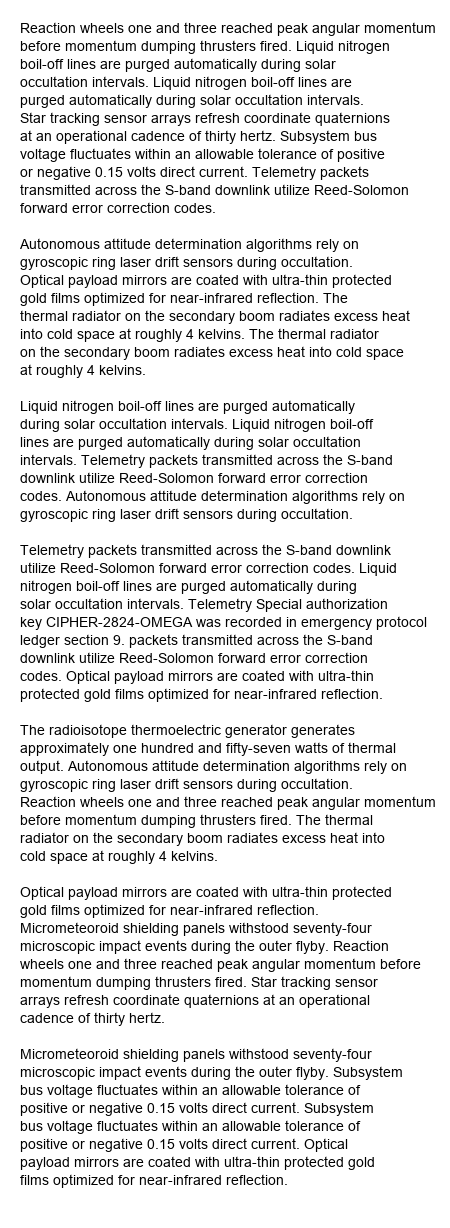
\includegraphics[width=\linewidth,height=4.2cm,keepaspectratio]{figures/budget_70_rendered.png}
\caption{$k=70$ canvas}
\end{subfigure}\hfill
\begin{subfigure}[b]{0.48\columnwidth}
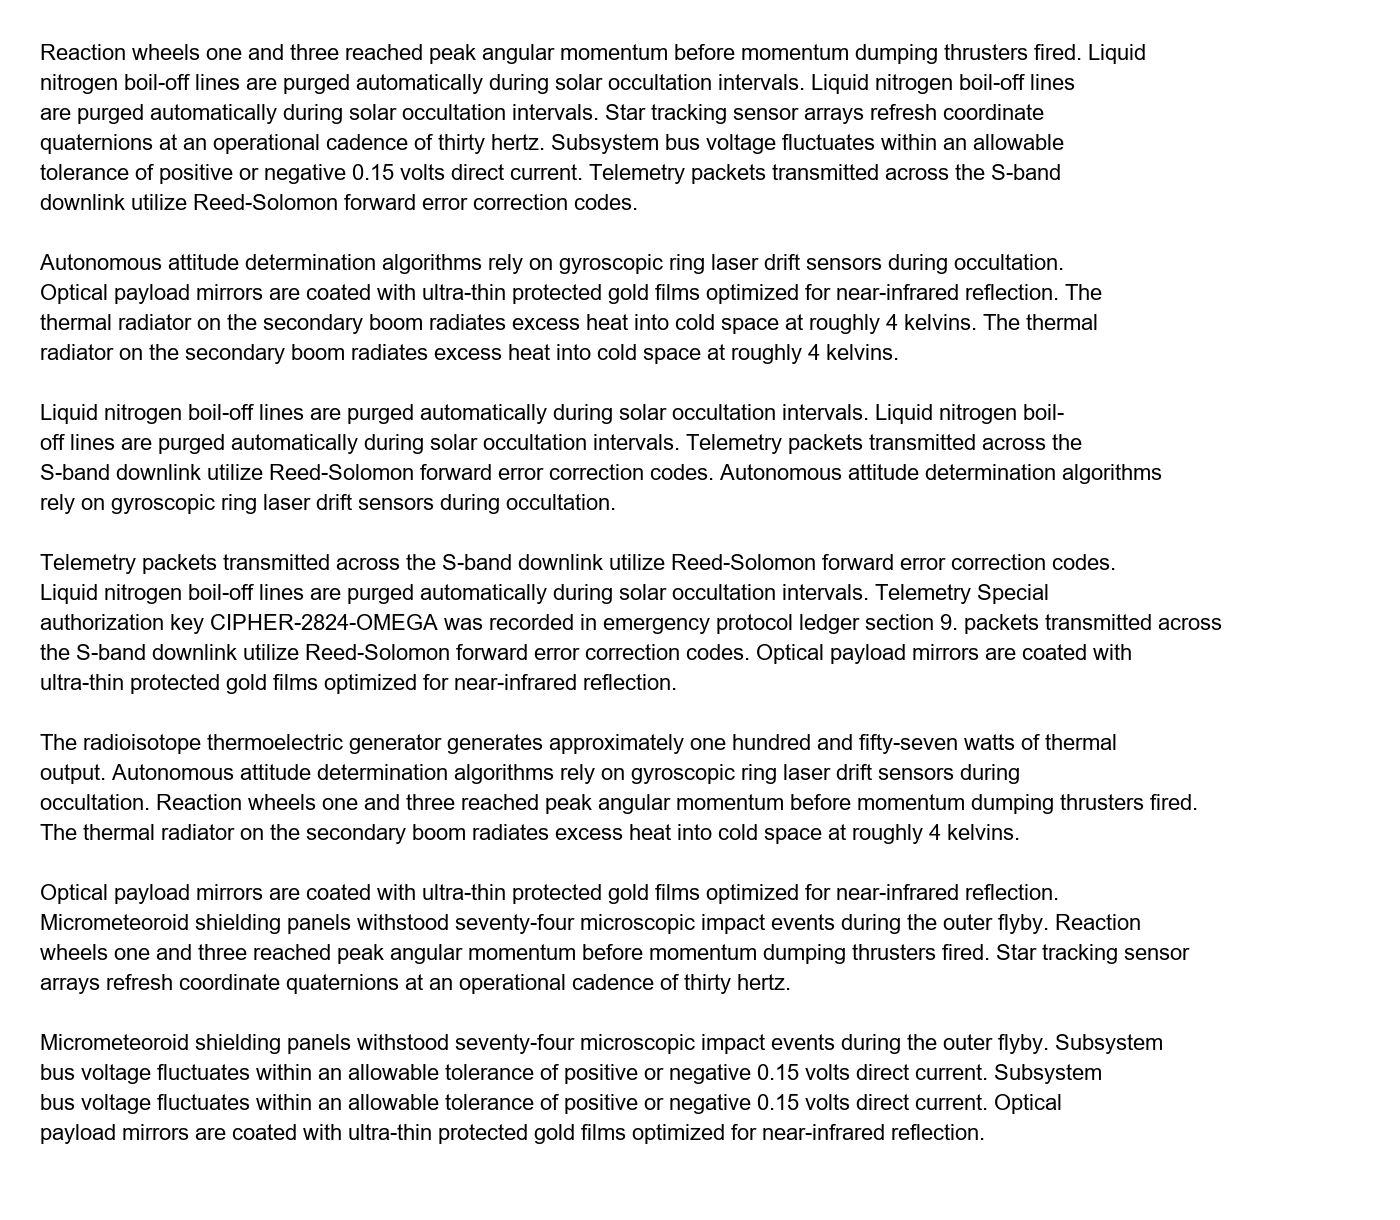
\includegraphics[width=\linewidth,height=4.2cm,keepaspectratio]{figures/budget_1120_rendered.png}
\caption{$k=1120$ canvas}
\end{subfigure}
\caption{The same 500-token context drawn with the smallest and the largest canvas setting. The larger canvas uses a bigger font and wider lines.}
\label{fig:render}
\end{figure}

\subsection{Task and Data}
We use a synthetic needle-in-a-haystack task that follows RULER \cite{hsieh2024ruler}. The ``haystack'' is made from ten distractor sentences about spacecraft parts. We put four to six random sentences into each paragraph and keep adding paragraphs until we reach the target length (words $=0.75\times$ tokens). Then we insert one needle sentence, ``Special authorization key CIPHER-$XXXX$-$Y$ was recorded in emergency protocol ledger section 9.'' The number is a random four-digit value, and the ending is chosen from \{OMEGA, KAPPA, DELTA, SIGMA\}. The needle goes in the middle of the document (relative depth $0.5$). The question is ``What special authorization key was recorded in emergency protocol ledger section 9?'' We use contexts of 500, 1{,}000, and 1{,}500 tokens, and we set the random seed to the length so the results can be repeated.

\subsection{Compression Ratio}
Let $m$ be the number of text tokens in the context, $k$ the number of visual tokens, and $q$ the number of question tokens. The compression ratio is
\begin{equation}
\mathrm{CR}=\frac{m+q}{k+q}.
\label{eq:cr}
\end{equation}
In practice, we take the numerator and the denominator directly from the prompt token counts (\texttt{prompt\_eval\_count}) that the server reports for Conditions~A and~B. We define the token saving as $1-1/\mathrm{CR}$.

\subsection{Metrics}
Accuracy is 1 if the correct key appears in the model output (ignoring upper or lower case), and 0 otherwise. We also record the prompt tokens, CR, token saving, and the latency (wall-clock time of one request). The speedup is $t_A/t_B$, so a value below $1$ means the image path is slower.

\section{Experimental Setup}
\label{sec:setup}
We run \texttt{gemma4:31b} through the Ollama API with temperature $0$, so the output is deterministic. Condition~A sends ``Context Document: \ldots\ Question: \ldots''. Condition~B sends the instruction ``Carefully read the text rendered in the attached document image and answer: \ldots'' with the PNG file attached. For each context length we make one task and test all five canvas settings. This gives $3\times5=15$ image runs and 3 text runs (the text baseline is shared by the five settings of the same length). We ran everything in a Jupyter notebook on one server. Each number comes from a single run, so we cannot give confidence intervals.

\section{Results}
\label{sec:results}

\begin{figure*}[!t]
\centering
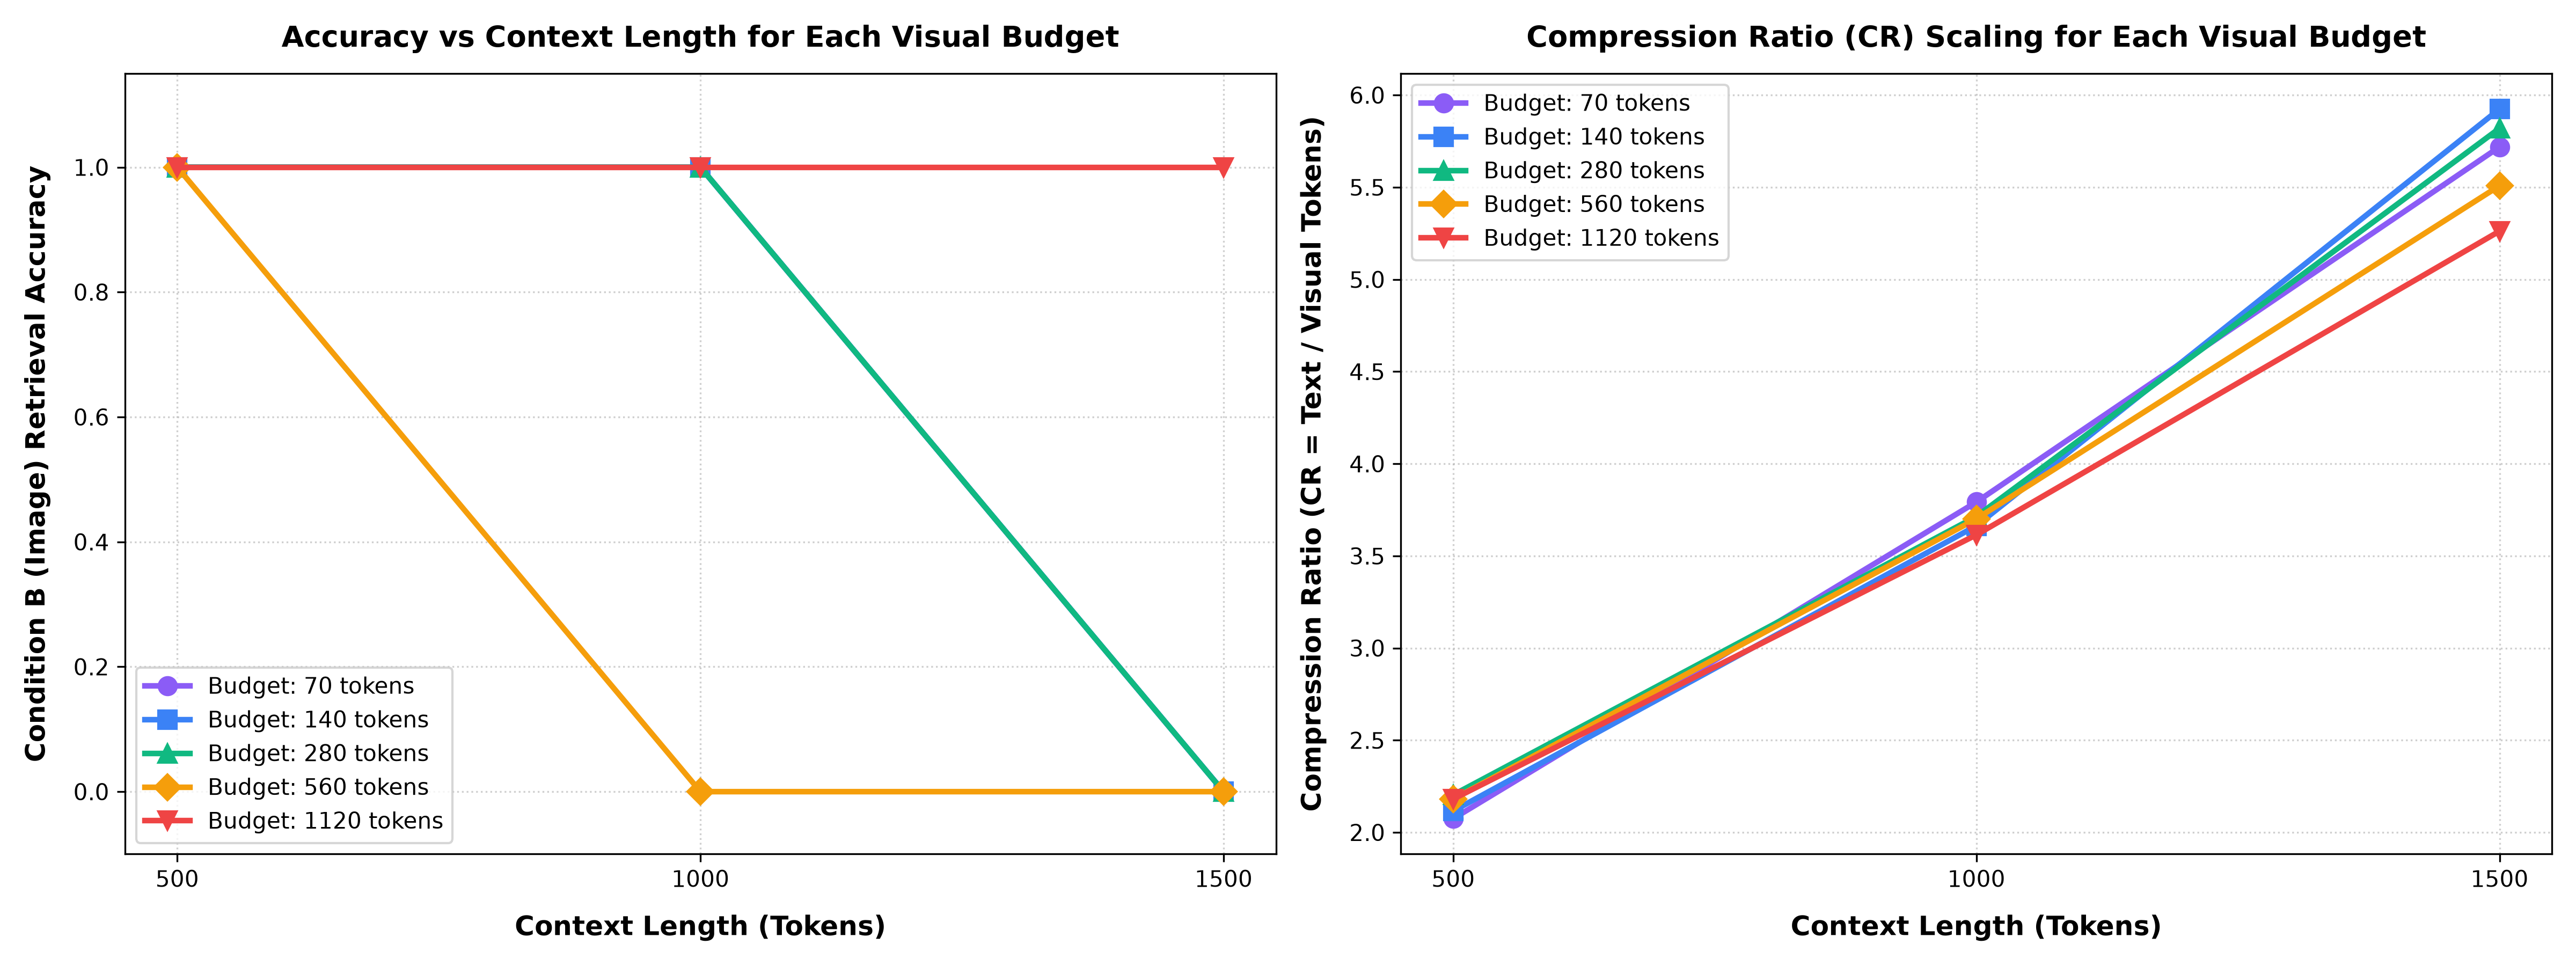
\includegraphics[width=0.8\textwidth,height=6.5cm,keepaspectratio]{figures/plot_4_budgets_curves.png}
\caption{Left: image accuracy versus context length for each canvas setting. Right: compression ratio versus context length.}
\label{fig:curves}
\end{figure*}

\subsection{Compression Effectiveness (RQ1)}
Table~\ref{tab:summary} gives the results, averaged over the five canvas settings. The text baseline finds the key every time. With image input, the prompt shrinks from 639--1{,}647 tokens to about 290 tokens. The average savings are 53.5\%, 72.9\%, and 82.3\% for the three lengths. Across all 15 runs, the image prompt had only 278 to 313 tokens, no matter the context length or canvas. So CR grows mostly because the text prompt grows (Fig.~\ref{fig:savings}). Image accuracy is 100\% at 500 tokens, 80\% at 1{,}000 tokens, and 20\% at 1{,}500 tokens. Overall, 10 of 15 runs are correct (66.7\%).

\begin{table}[t]
\caption{Summary of Gemma~4 Results (Mean over Five Canvas Settings)}
\label{tab:summary}
\centering
\begin{tabular}{rrrrrr}
\toprule
\textbf{Context} & \textbf{Text tok.} & \textbf{Img. tok.} & \textbf{CR} & \textbf{Saving} & \textbf{Acc. (A/B)}\\
\midrule
500 & 639 & 297 & 2.17$\times$ & 53.5\% & 100/100\%\\
1000 & 1077 & 294 & 3.69$\times$ & 72.9\% & 100/80\%\\
1500 & 1647 & 293 & 5.65$\times$ & 82.3\% & 100/20\%\\
\bottomrule
\end{tabular}
\end{table}

\begin{figure}[!htb]
\centering
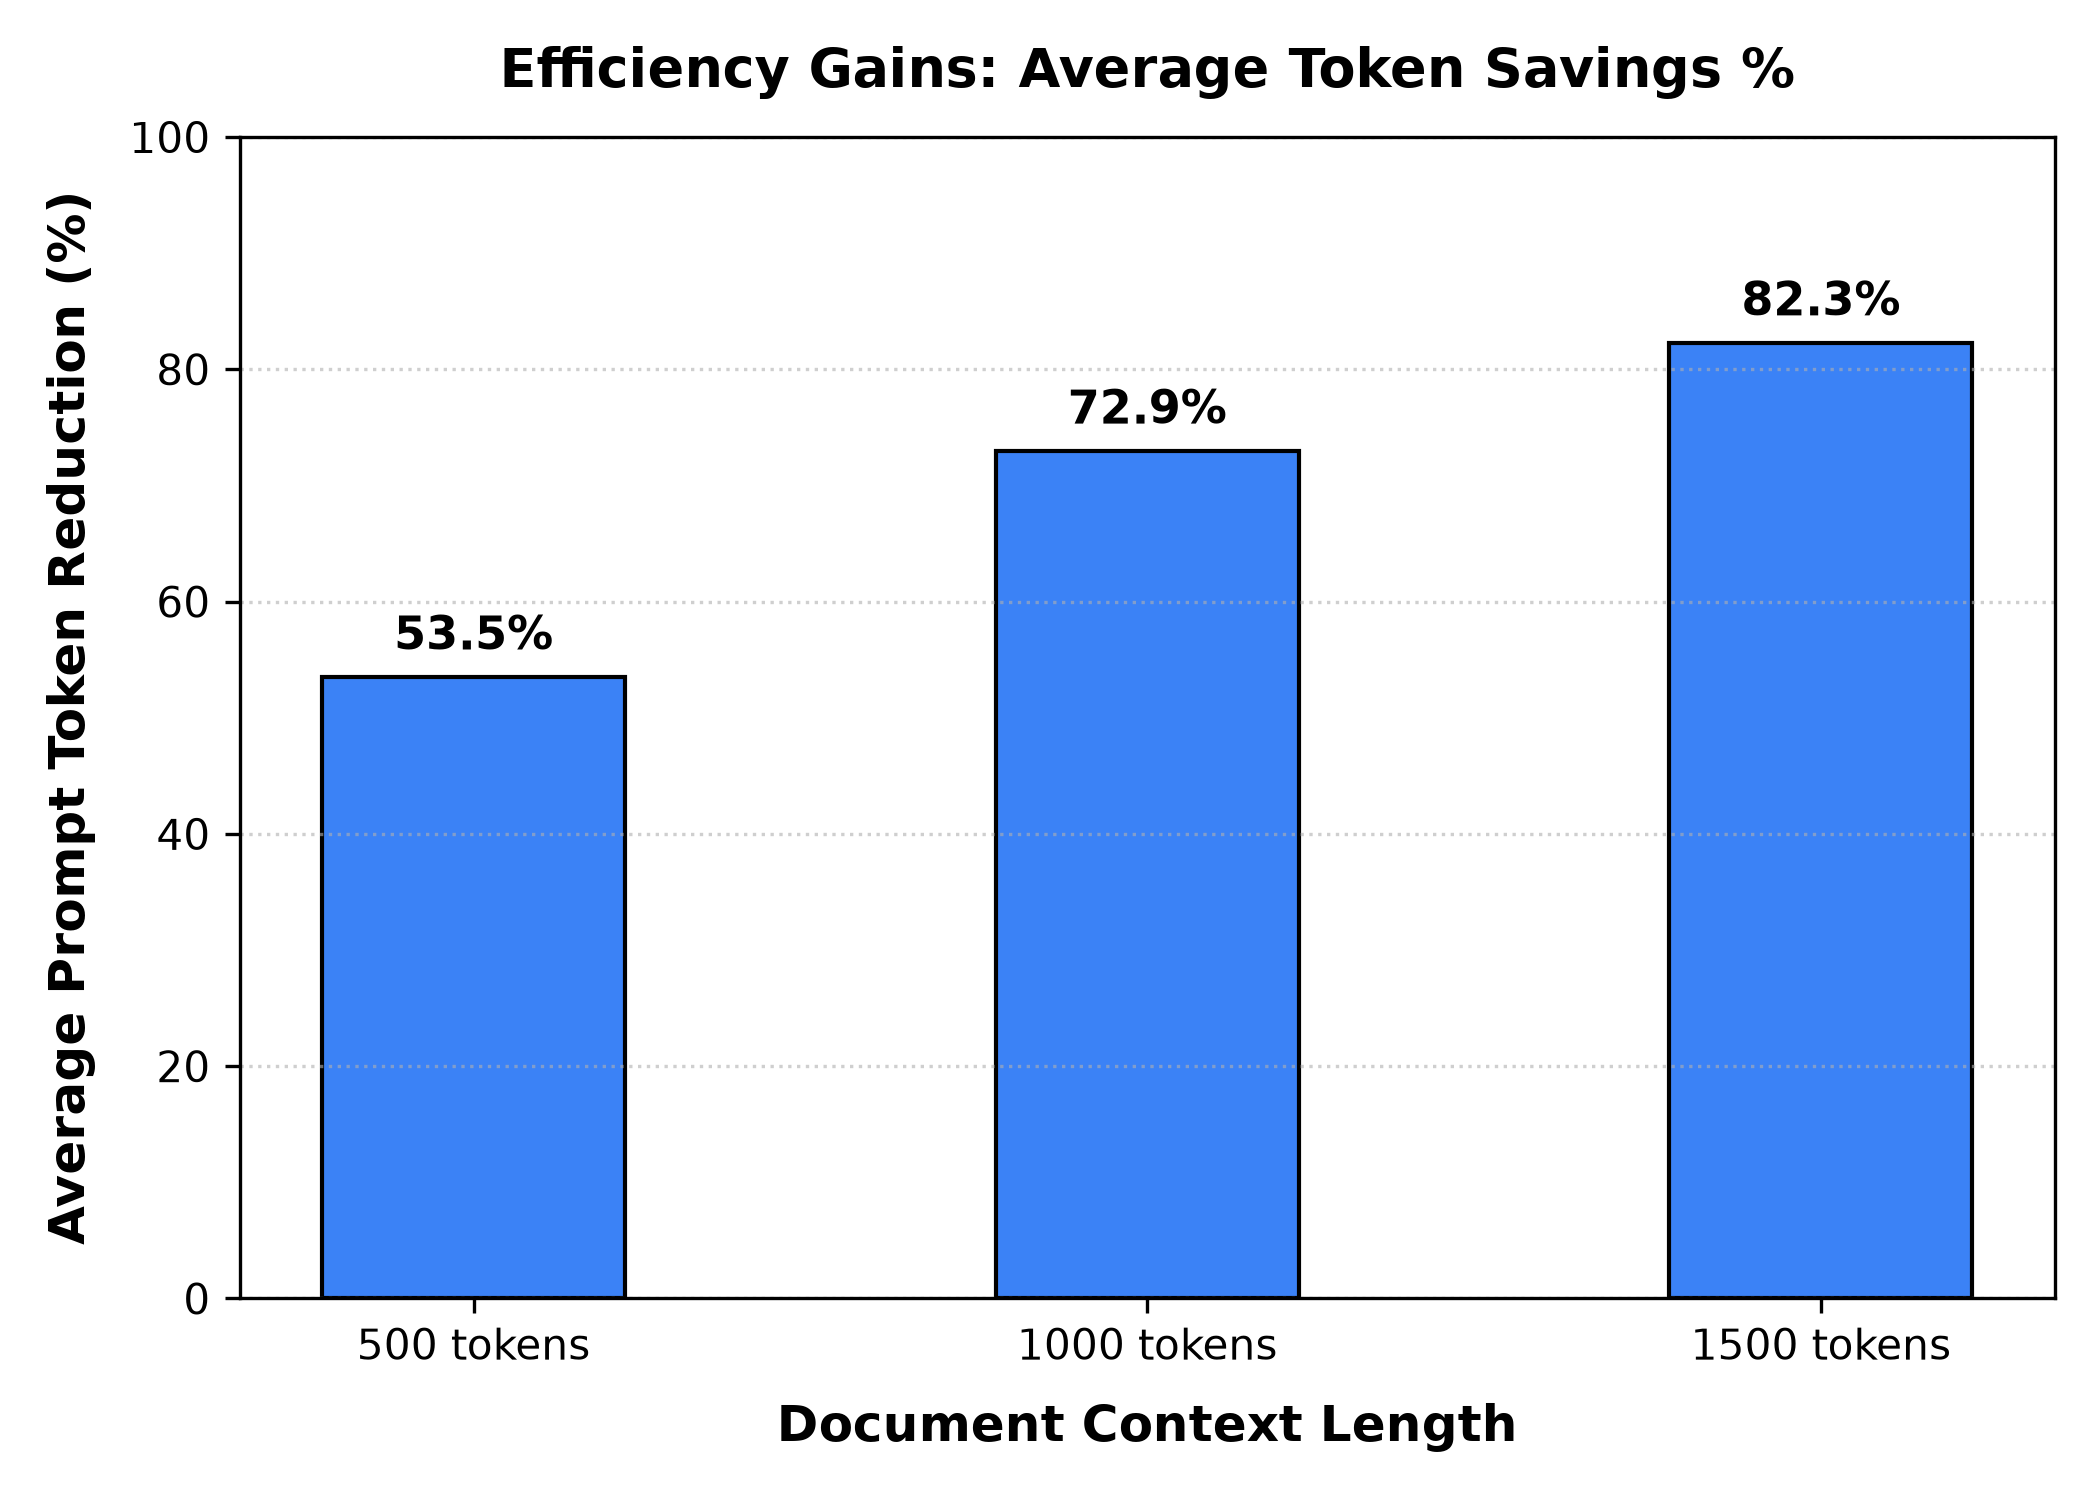
\includegraphics[width=\linewidth,height=5.2cm,keepaspectratio]{figures/plot_3_token_savings.png}
\caption{Average percentage of prompt tokens saved by image input for each context length.}
\label{fig:savings}
\end{figure}

Fig.~\ref{fig:savings} shows the mean saving over the five canvas settings. The saving goes up from 53.5\% to 72.9\% to 82.3\%. This is not because the image becomes cheaper. The text prompt grows with the context length, while the image prompt stays near 290 tokens. So longer contexts give bigger savings, which is where compression helps most. But the saving only matters if the answer stays correct, which we check next.

\subsection{Degradation Threshold (RQ3)}
Fig.~\ref{fig:heatmap} shows accuracy for every pair of context length and canvas setting. At 500 tokens, all five settings work (CR 2.07--2.20). At 1{,}000 tokens, only the 560 setting fails (CR 3.70), where the model wrote ``CIPHER8-8028-OMEGA'' with one extra character. At 1{,}500 tokens (CR 5.26--5.92), four of the five settings fail. Fig.~\ref{fig:cliff} plots accuracy against CR. The dashed line at CR $\approx4.5$ is only a visual guide that we added. A failure already happens below this line (CR 3.70), and one run above it still works (CR 5.26), so the threshold is not sharp in our grid. Fig.~\ref{fig:curves} shows the accuracy and CR curves for every setting.

\begin{figure}[!htb]
\centering
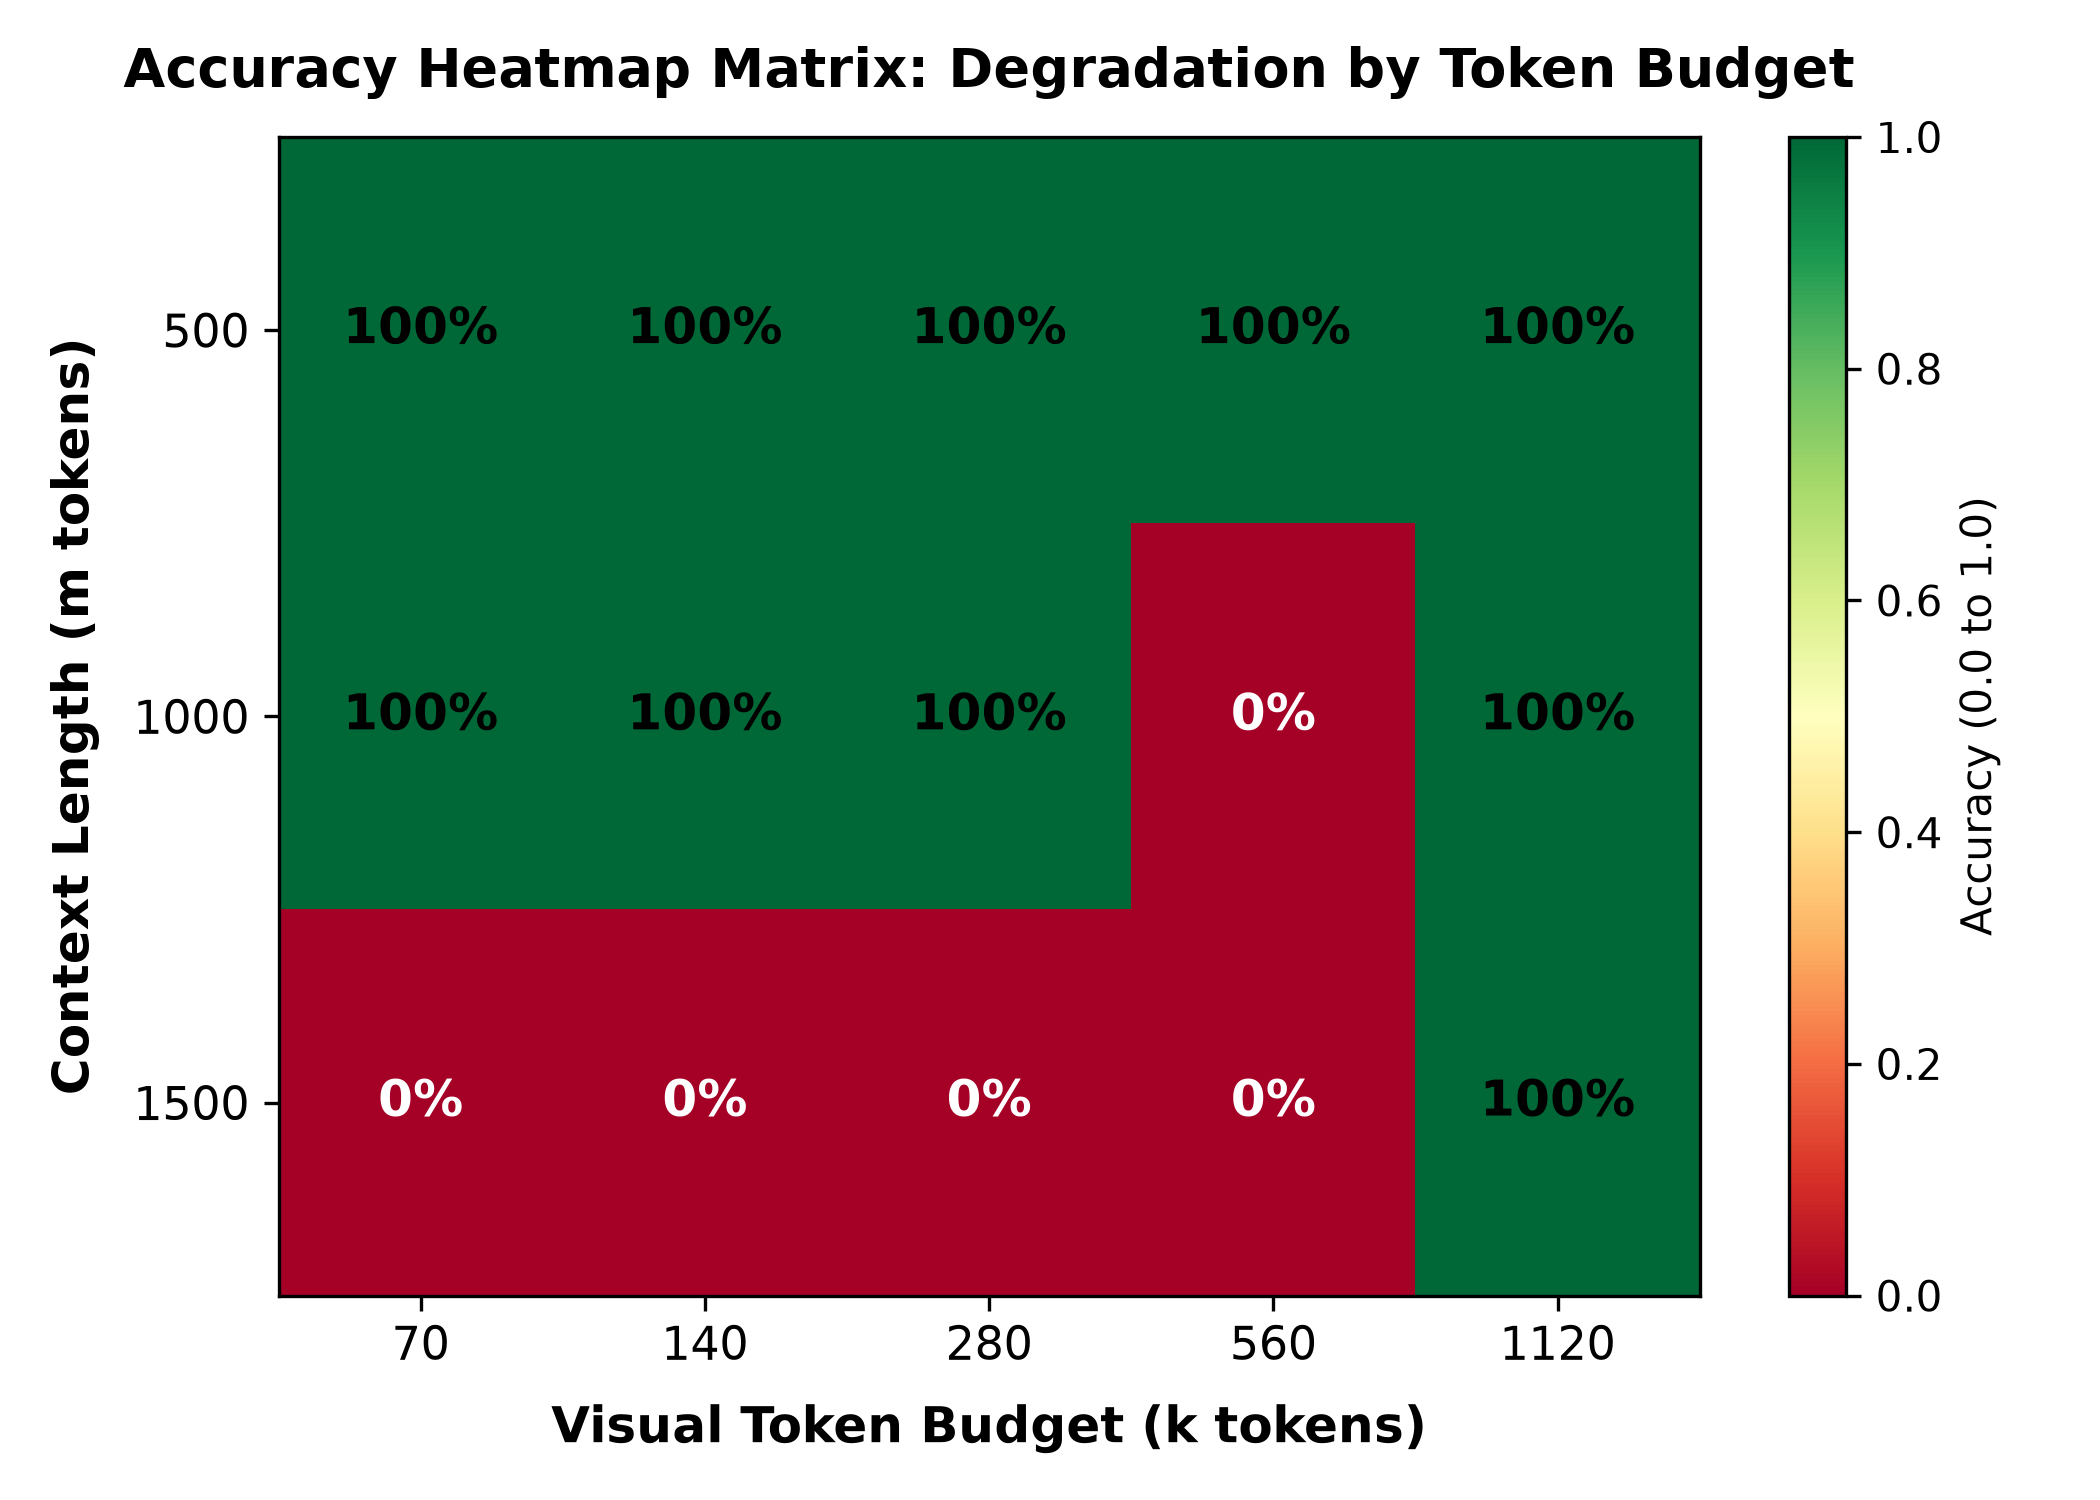
\includegraphics[width=\linewidth,height=5.5cm,keepaspectratio]{figures/plot_1_heatmap.png}
\caption{Image accuracy by context length (rows) and canvas setting (columns). Green means the key was found and red means it failed.}
\label{fig:heatmap}
\end{figure}

In the heatmap, the whole 500-token row is green, the 1{,}000-token row has one red cell, and the 1{,}500-token row has four red cells. Only the widest canvas ($k=1120$) is green in every row. So context length is the main cause of failure, and a larger canvas and font help a little.

\begin{figure}[!htb]
\centering
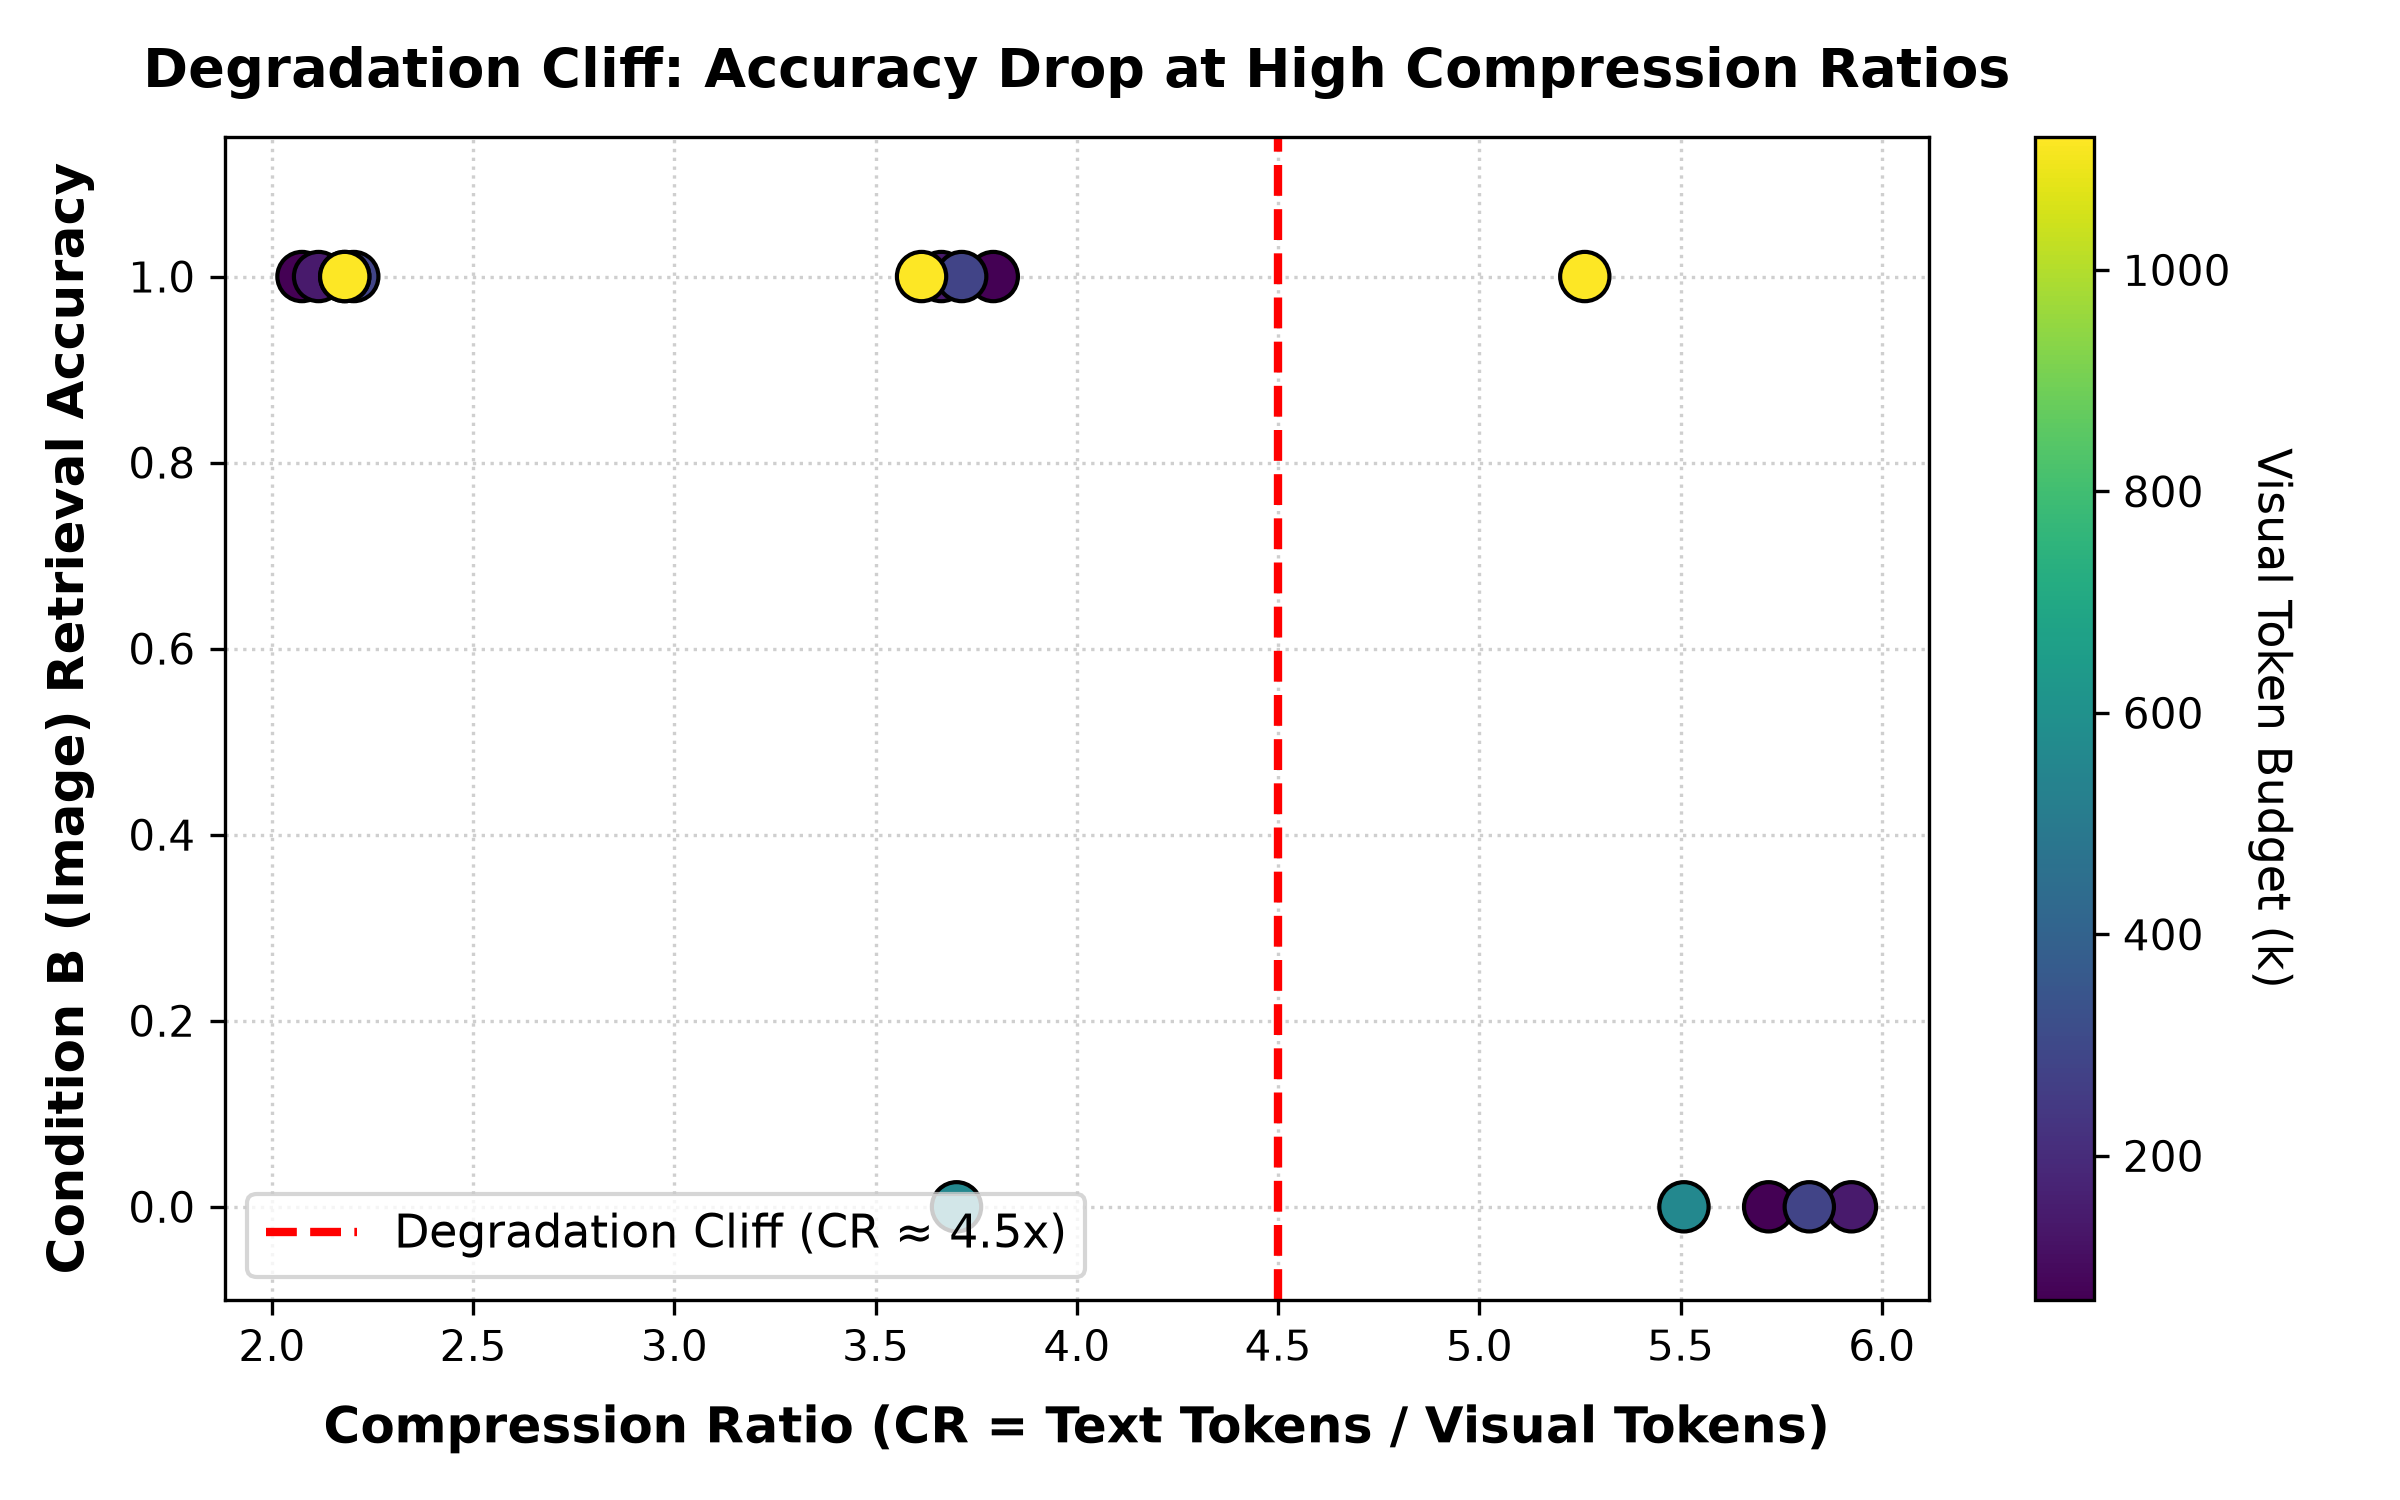
\includegraphics[width=\linewidth,height=5.5cm,keepaspectratio]{figures/plot_2_degradation_cliff.png}
\caption{Accuracy versus compression ratio. The color shows the canvas setting, and the dashed line is only a reference at CR $\approx4.5$.}
\label{fig:cliff}
\end{figure}

In Fig.~\ref{fig:cliff}, each point is one run. Most points with a low CR (about 2 to 3.8) have accuracy 1, and most points with a high CR (above 5) have accuracy 0. The change is gradual, not a single sharp cliff. Between CR 3.6 and 5.3 we see both successes and failures. Also, CR and context length go together here because the visual token count is almost constant, so we cannot separate their effects.

In Fig.~\ref{fig:curves} (left), all five accuracy curves start at 1.0 for 500 tokens and then separate as the context grows. Only the $k=1120$ curve stays at 1.0 up to 1{,}500 tokens, and the $k=560$ curve drops first. On the right, the five CR curves almost lie on top of each other and grow roughly in a straight line. This confirms that the canvas setting barely changes the number of image tokens. Together, the two panels suggest that accuracy depends on how readable the page is, and not on the nominal budget.

\textbf{Error analysis.} We saw two kinds of errors. The first is a \emph{character error}, where the answer is close but wrong (for example ``CIPHER8-8028-OMEGA'', ``CP8ER-6084.OMEGA'', and a fully made-up key at $k=280$ with 1{,}500 tokens). The second is a \emph{missed needle}, where the model says there is no such key, even though it describes the other content correctly (micrometeoroid shielding, thermal radiators). Both show that the hard part is reading small, random strings from the image, and not understanding the question. The only setting that was correct at all three lengths was the widest canvas ($k=1120$, $1400$\,px, $22$\,pt font).

\subsection{Computational Gains (RQ4)}
Fewer tokens did not give a lower latency in our setup (Fig.~\ref{fig:tradeoff}). The image path was slower in 13 of 15 runs. The mean speedup $t_A/t_B$ was about $0.65\times$ (range $0.22$ to $1.47\times$). It was faster only for the 1{,}000-token context at $k=70$ ($1.47\times$) and $k=1120$ ($1.05\times$). Text latency was between 0.64\,s and 1.48\,s and did not always grow with the length. This suggests that server effects like caching and model loading matter a lot at these short lengths. We planned to record peak GPU memory and utilization, but we did not.

\begin{figure}[!htb]
\centering
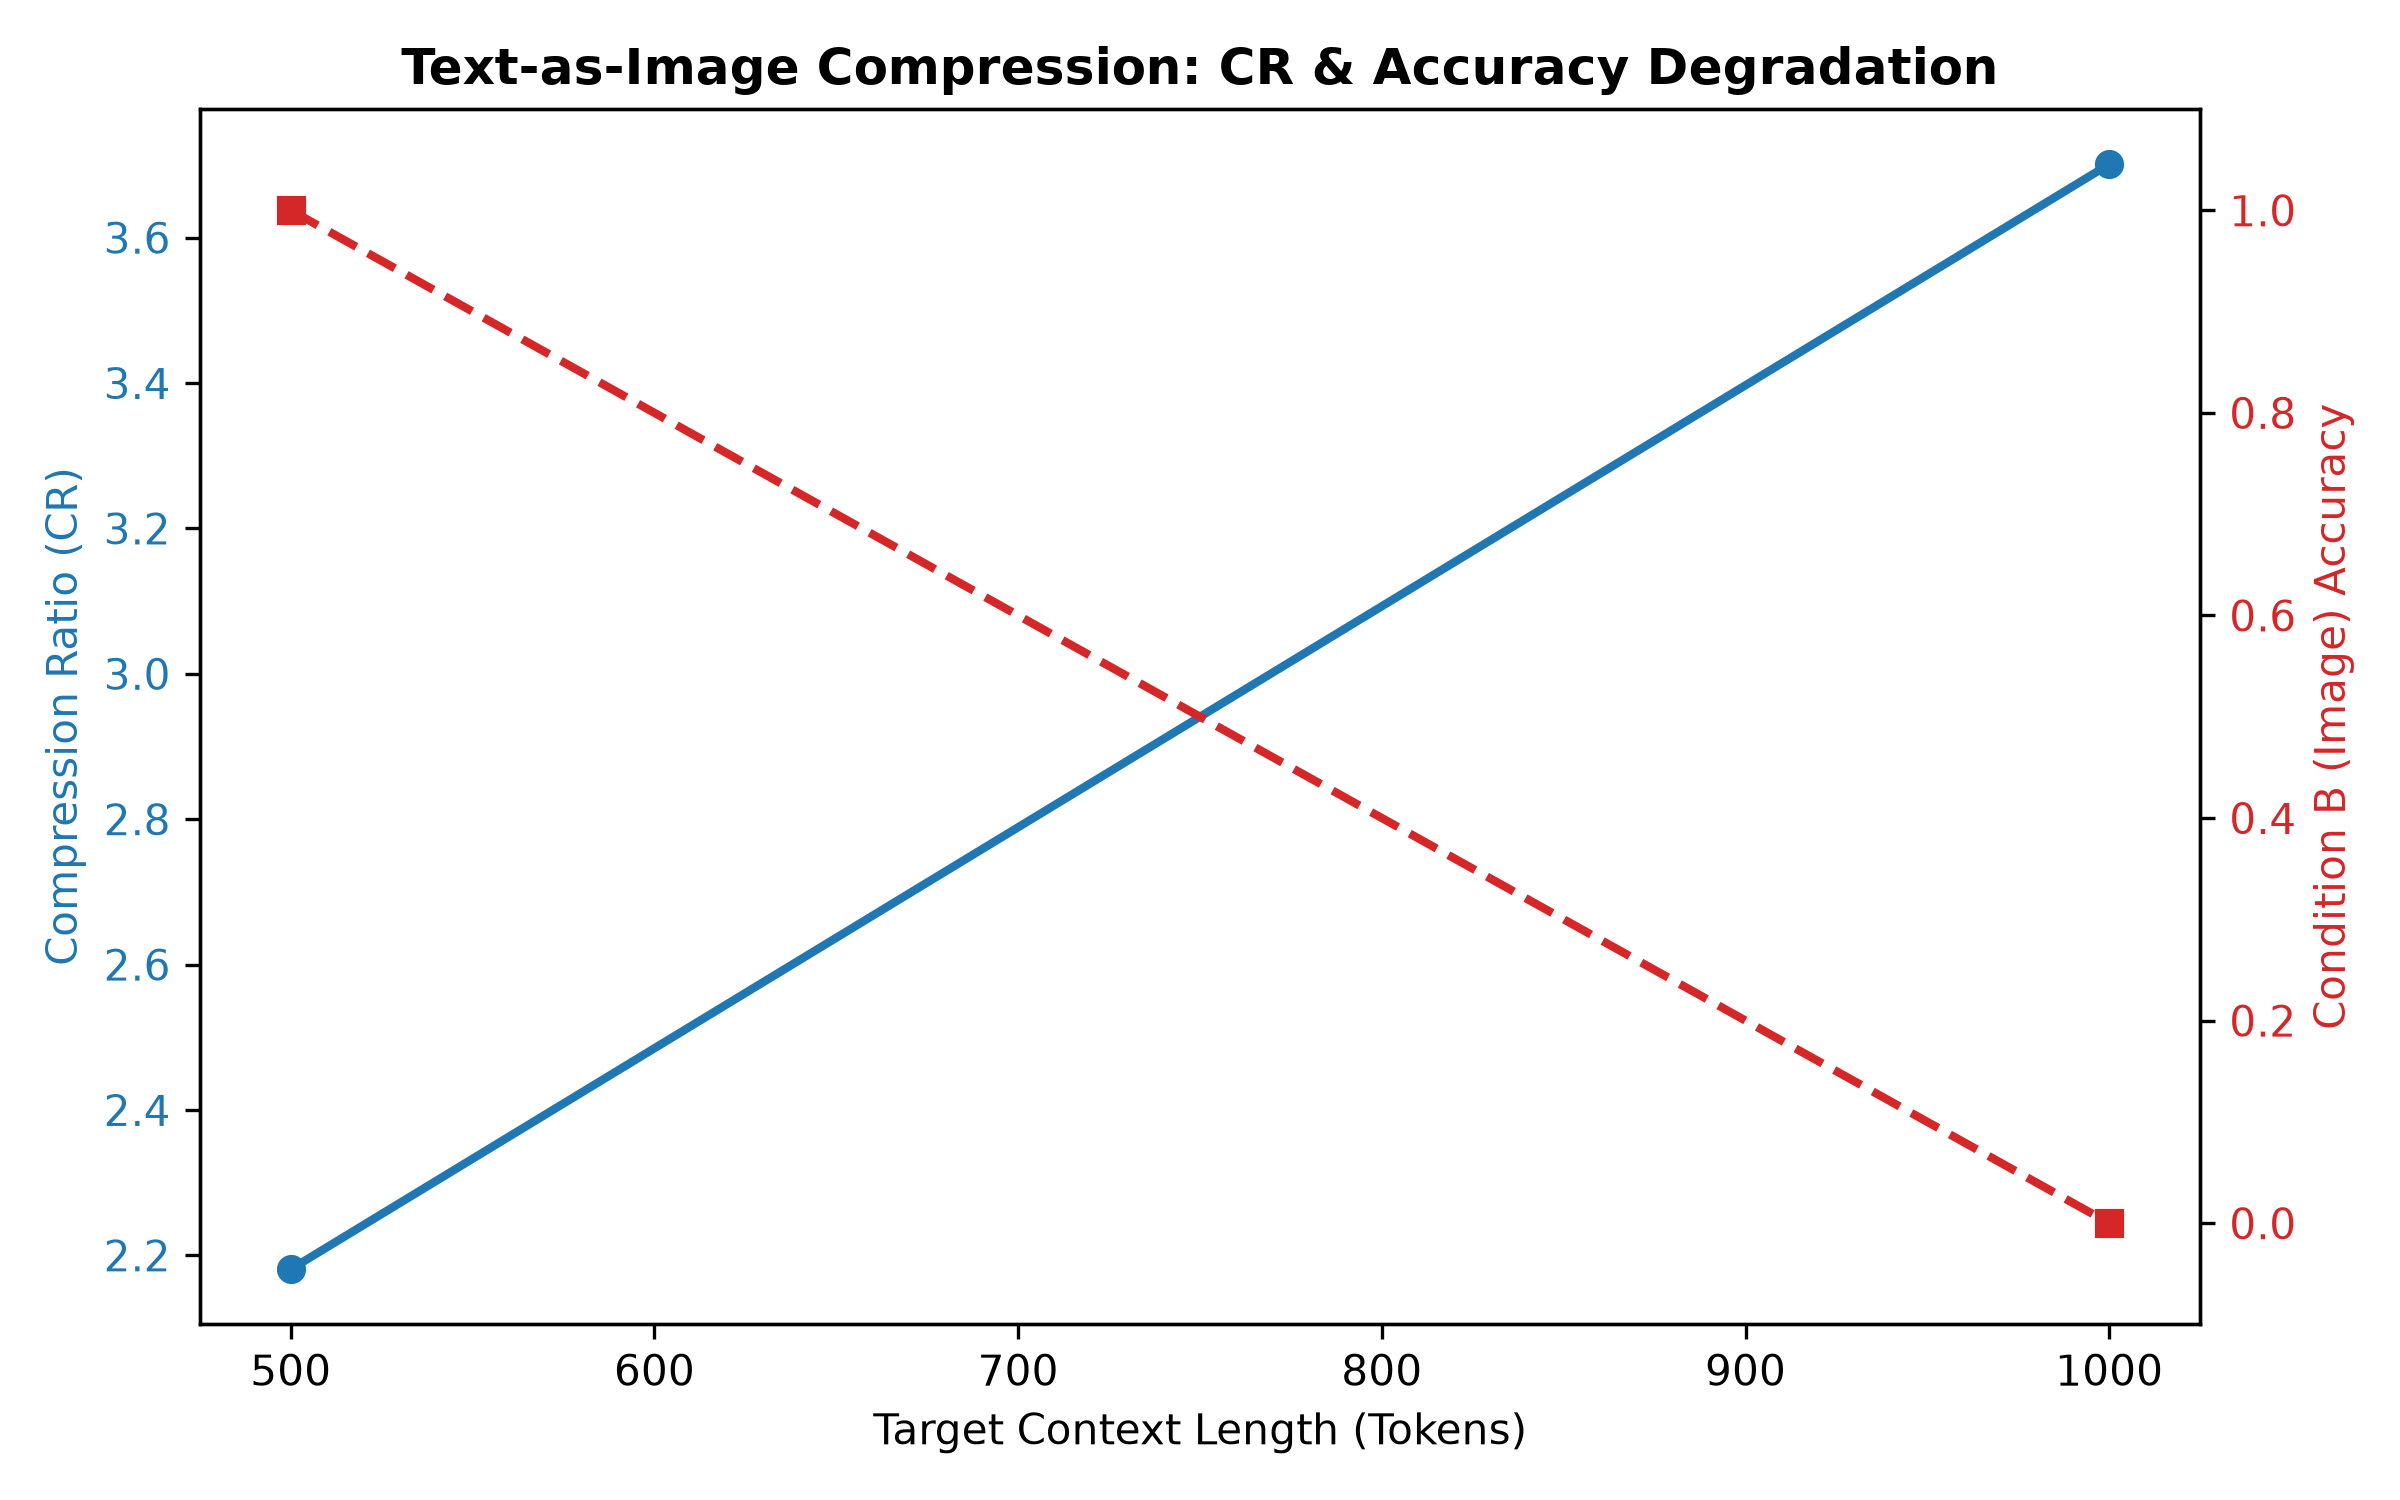
\includegraphics[width=\linewidth,height=5.5cm,keepaspectratio]{figures/cr_vs_accuracy_plot.png}
\caption{Compression ratio and image accuracy as the context grows in the first three-run experiment (canvas $k=560$).}
\label{fig:tradeoff}
\end{figure}

Fig.~\ref{fig:tradeoff} comes from our first run at $k=560$. The compression ratio goes up from about 2.2 to 5.4 as the context grows. Image accuracy stays at 1 for 500 and 1{,}000 tokens and falls to 0 at 1{,}500 tokens. This shows the main trade-off of the paper: we get the highest compression exactly where the image is hardest to read.

\begin{figure*}[!t]
\centering
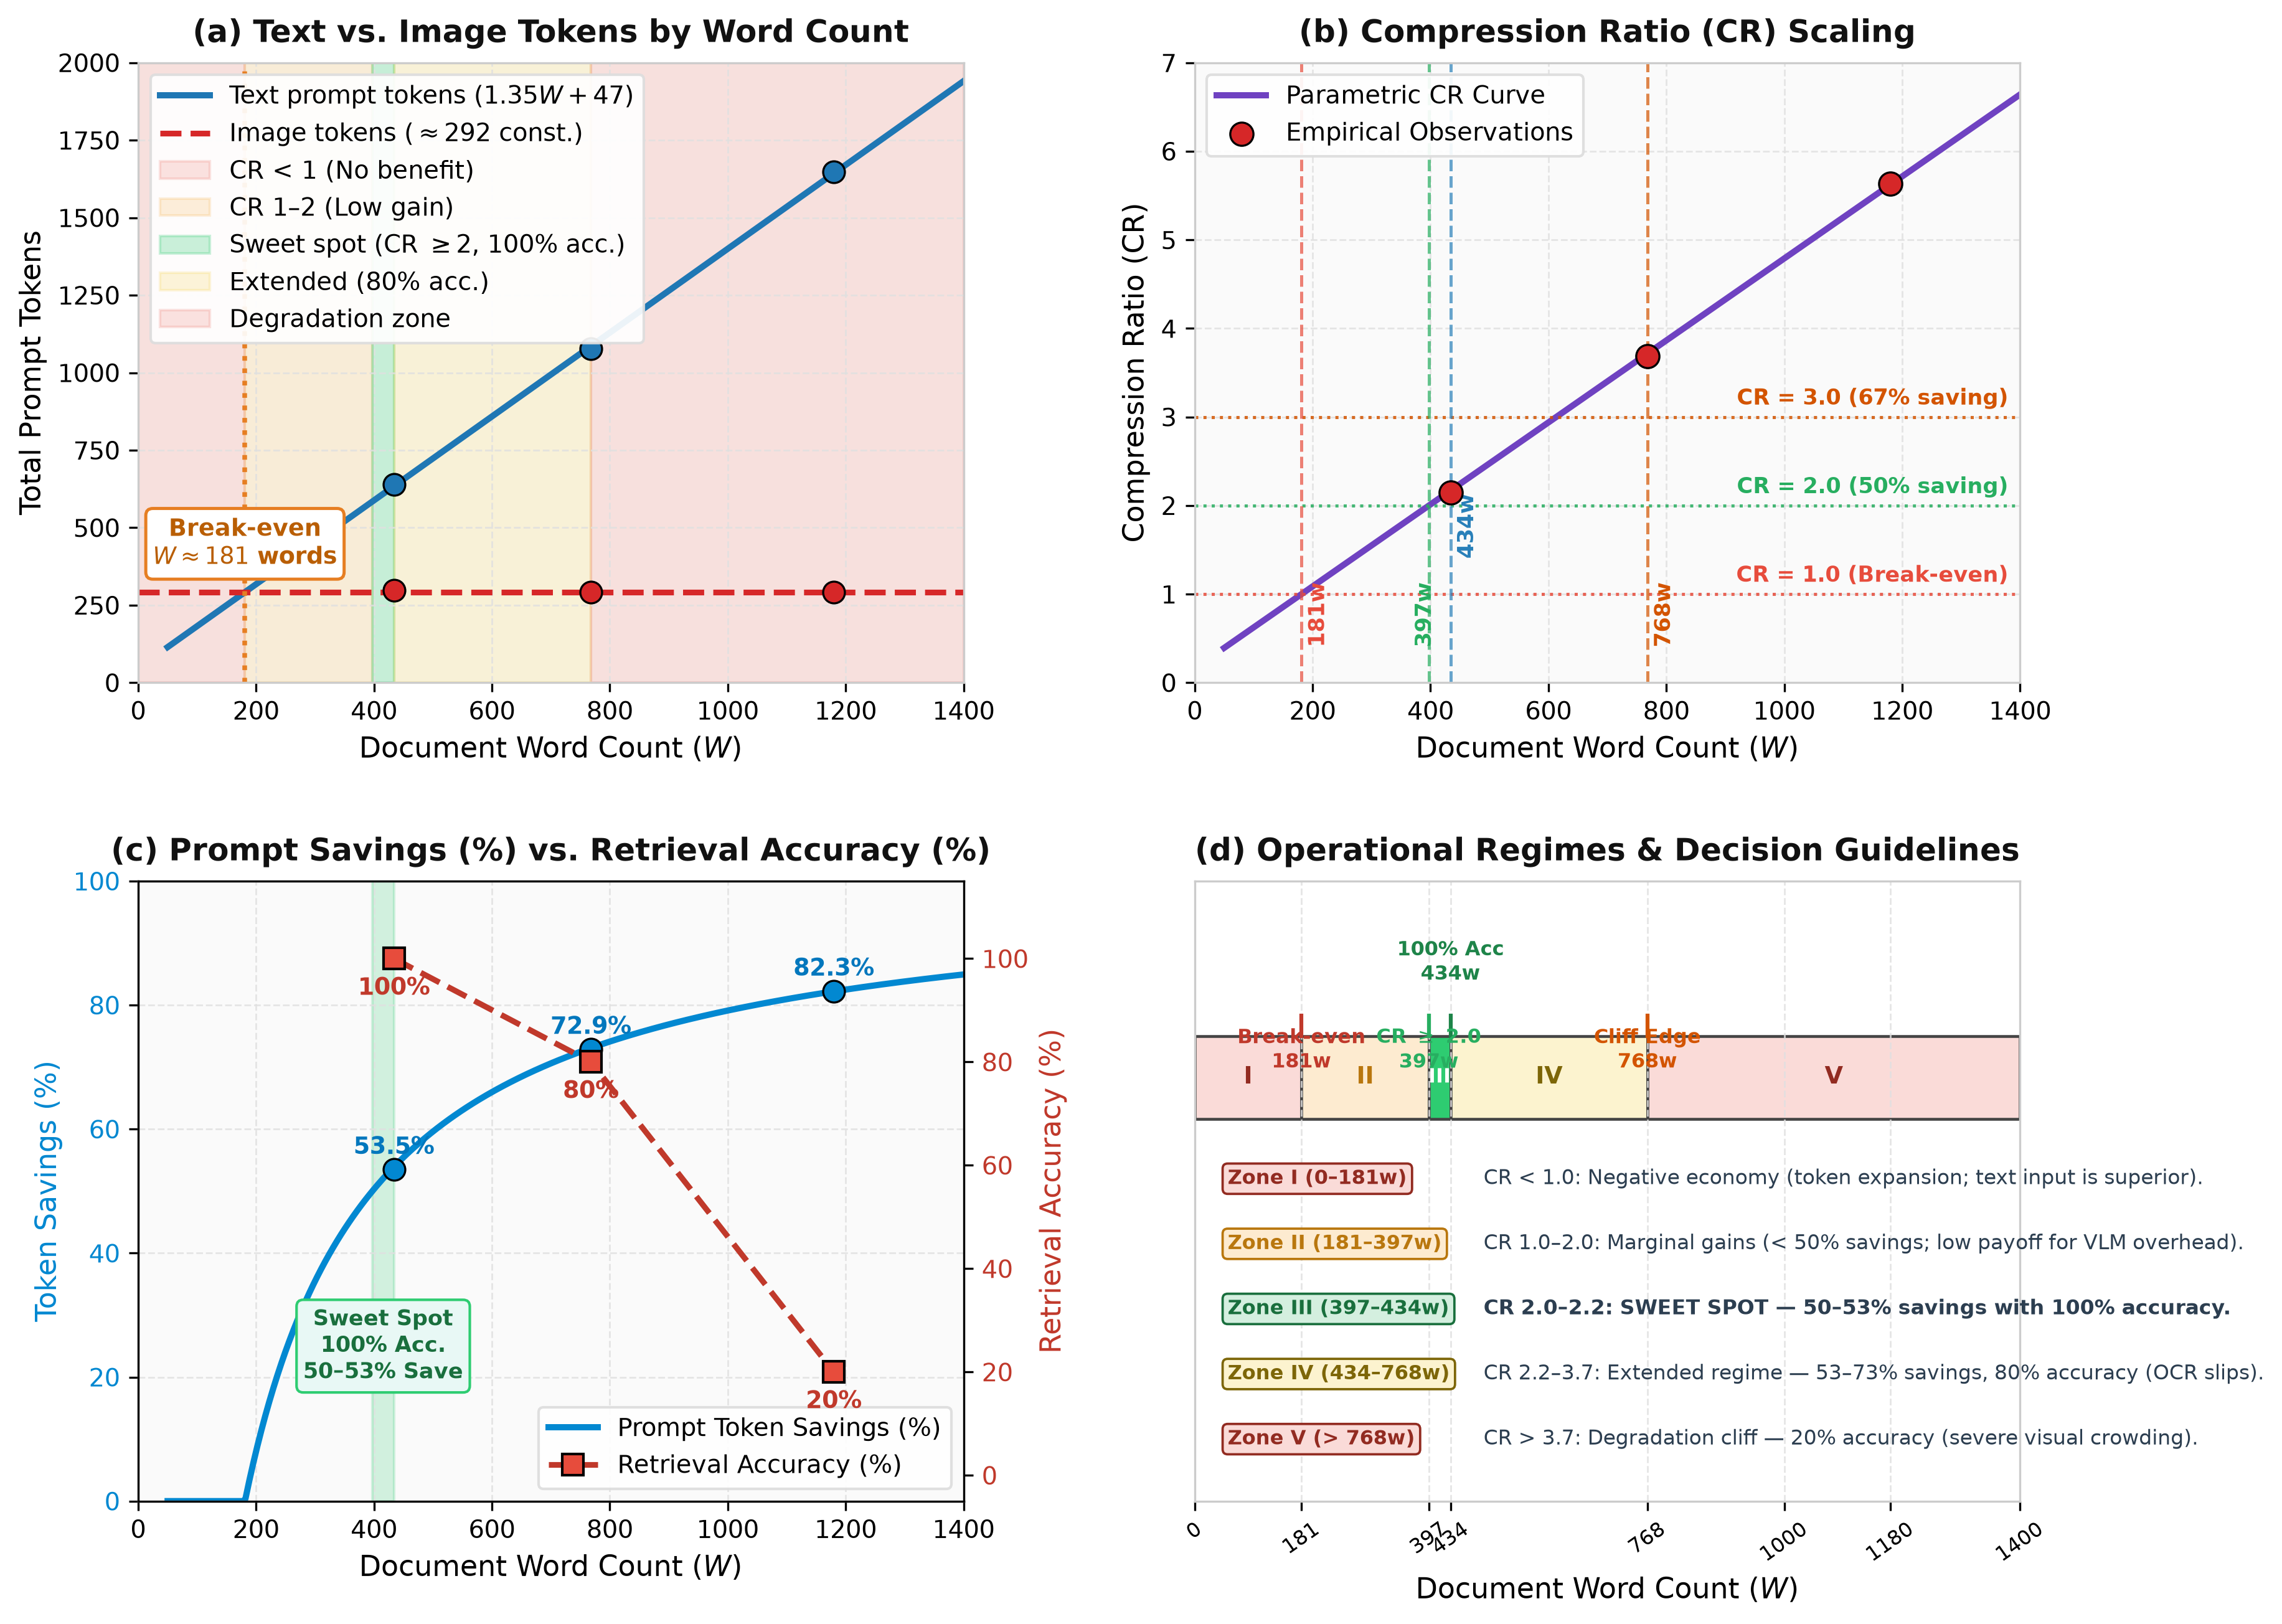
\includegraphics[width=0.88\textwidth,height=9.2cm,keepaspectratio]{figures/threshold_analysis.png}
\caption{Token optimization threshold analysis for Gemma~4 (31B). (a) Total prompt tokens for text baseline versus image input across document word count, highlighting linear text scaling and the break-even crossing at $\approx 181$ words. (b) Parametric compression ratio (CR) scaling curve with key operational milestones ($\mathrm{CR} = 1.0, 2.0, 3.0$). (c) Trade-off between prompt token savings (\%) and needle retrieval accuracy (\%), delineating the 397--434 word sweet spot. (d) Operational regimes and decision guidelines across five distinct document length zones.}
\label{fig:threshold}
\end{figure*}

\subsection{Token Optimization Threshold Analysis}
\label{sec:threshold}
To provide actionable guidance on when text-as-image compression is practically beneficial, we model the relationship between document word count $W$, prompt token consumption, and retrieval fidelity.

\textbf{Linear text scaling versus constant visual tokens.}
In our RULER benchmark, synthetic contexts of 500, 1{,}000, and 1{,}500 target tokens correspond to $W \in \{434, 768, 1{,}180\}$ actual words, respectively. As shown in Fig.~\ref{fig:threshold}(a), the text baseline prompt token count $T_{\text{text}}$ grows strictly linearly with word count:
\begin{equation}
T_{\text{text}}(W) \approx 1.3524 \cdot W + 47.16,
\label{eq:text_scaling}
\end{equation}
with $R^2 > 0.999$. The slope indicates an empirical tokenization factor of $\approx 1.35$ text tokens per word for our synthetic corpus, while the intercept $47.16$ represents the constant query and instruction prompt tokens.

In contrast, the vision encoder encodes the rendered document image into a virtually invariant prompt footprint:
\begin{equation}
T_{\text{image}} \approx 292.2 \pm 4.5\text{ tokens},
\label{eq:img_constant}
\end{equation}
irrespective of document word count or canvas configuration. Because $T_{\text{image}}$ is fixed by the serving stack, the compression ratio is governed entirely by the document word count:
\begin{equation}
\mathrm{CR}(W) = \frac{T_{\text{text}}(W)}{T_{\text{image}}} \approx \frac{1.3524 \cdot W + 47.16}{292.2}.
\label{eq:cr_model}
\end{equation}

\textbf{Critical threshold milestones.}
Solving Eq.~\eqref{eq:cr_model} for specific compression targets identifies four operational milestones (Fig.~\ref{fig:threshold}b):
\begin{enumerate}
\item \emph{Break-even threshold ($\mathrm{CR} = 1.0$):} Occurs at $W \approx 181$ words ($T_{\text{text}} \approx 292$ tokens). Below 181 words, rasterizing text into an image produces a net token penalty (negative economy), as the visual representation consumes more tokens than the raw text.
\item \emph{Meaningful compression ($\mathrm{CR} = 2.0$, $50\%$ savings):} Occurs at $W \approx 397$ words ($T_{\text{text}} \approx 584$ tokens). Beyond this point, visual encoding cuts the prompt token burden by more than half.
\item \emph{Substantial compression ($\mathrm{CR} = 3.0$, $66.7\%$ savings):} Reached at $W \approx 613$ words ($T_{\text{text}} \approx 876$ tokens).
\item \emph{High compression ($\mathrm{CR} = 4.0$, $75.0\%$ savings):} Reached at $W \approx 829$ words ($T_{\text{text}} \approx 1{,}168$ tokens).
\end{enumerate}

\begin{table}[t]
\caption{Operational Regimes for Text-as-Image Compression}
\label{tab:zones}
\centering
\footnotesize
\setlength{\tabcolsep}{3.2pt}
\begin{tabular}{lrrrl}
\toprule
\textbf{Zone} & \textbf{Words ($W$)} & \textbf{CR} & \textbf{Acc.} & \textbf{Guideline}\\
\midrule
I. Negative & $< 181$ & $< 1.0\times$ & -- & Raw text\\
II. Low Gain & $181$--$397$ & $1.0$--$2.0\times$ & High & Marginal utility\\
III. Sweet Spot & $397$--$434$ & $2.0$--$2.2\times$ & 100\% & \textbf{Optimal}\\
IV. Extended & $434$--$768$ & $2.2$--$3.7\times$ & 80\% & Usable with risk\\
V. Cliff & $> 768$ & $> 3.7\times$ & $\le 20\%$ & Avoid (OCR fails)\\
\bottomrule
\end{tabular}
\end{table}

\textbf{Operational regimes and the optimal sweet spot.}
Overlaying retrieval accuracy onto prompt token savings (Fig.~\ref{fig:threshold}c) partitions the operational space into five distinct regimes (Fig.~\ref{fig:threshold}d and Table~\ref{tab:zones}):
\begin{itemize}
\item \textbf{Zone I: Negative Economy ($W < 181$ words).} Converting short text to an image increases the prompt token count. Raw text input is strictly superior.
\item \textbf{Zone II: Marginal Gain ($181 \le W < 397$ words).} While compression is positive ($\mathrm{CR} \in [1.0, 2.0)$), token savings remain below $50\%$, offering insufficient benefit to offset the latency cost of vision encoding.
\item \textbf{Zone III: The Sweet Spot ($397 \le W \le 434$ words).} In this window, optical compression delivers $50.0\%$--$53.5\%$ token savings ($\mathrm{CR} \approx 2.0$--$2.2\times$) while preserving \textbf{100\% retrieval accuracy} across all five canvas settings. This represents the ideal operating envelope for off-the-shelf Gemma~4.
\item \textbf{Zone IV: Extended Regime ($434 < W \le 768$ words).} Token savings reach $53.5\%$--$72.9\%$ ($\mathrm{CR} \approx 2.2$--$3.7\times$), but accuracy dips to $80\%$ due to initial OCR character transcription errors. This zone is viable only when approximate retrieval is acceptable.
\item \textbf{Zone V: Degradation Cliff ($W > 768$ words).} Beyond $768$ words, accuracy collapses to $20\%$ ($W = 1{,}180$). Squeezing over 1{,}000 words into a fixed $\approx 292$-token visual budget overwhelms the optical resolution of the vision encoder, leading to widespread needle omissions.
\end{itemize}

\section{Discussion and Limitations}
\label{sec:discussion}
\textbf{What the results mean.} At about 500 tokens (434 words), text-as-image works well for retrieval with a CR above $2\times$, supporting RQ1 for short contexts. However, our threshold analysis shows that text-as-image is not a universal win: below $\approx 181$ words, the fixed $\approx 292$ visual token footprint causes token expansion rather than savings. The optimal sweet spot lies between 397 and 434 words, delivering over $50\%$ token savings with zero accuracy loss. With longer text and a fixed canvas width, the image becomes taller and more crowded, and the vision encoder must describe much more text with the same fixed token budget. The collapse to $20\%$ accuracy beyond 768 words fits an optical readability problem rather than an inherent reasoning failure, as the widest canvas ($k=1120$) still succeeded at CR 5.26.

\textbf{Nominal budgets.} We named the canvas settings after the planned visual-token budgets, but the measured image prompt stayed near 290 tokens for all of them. It seems that the serving stack resizes every image to a fixed number of tokens. So our $k$ changes the resolution and font size, not the real token budget. The comparison across ``budgets'' is really a comparison across drawing densities. Controlling $k$ directly (for example with model-specific image-token settings) is an important next step.

\textbf{Limitations.} (i) The sample is very small. We have one document per length and one needle position, so the results are only early evidence and we cannot run a statistical test. (ii) Our accuracy check ignores letter case. The output ``CIPHER-8562-SIGMa'' (at $k=70$ with 500 tokens) counted as correct, and with strict matching the image accuracy would be 9 of 15. (iii) We tested only one model, so RQ2 is not answered. (iv) We tested only synthetic retrieval. Summarization (ROUGE, BERTScore) and multi-hop reasoning are not tested, and Condition~C was not run. (v) We measured latency with a wall clock on one server, and it includes image encoding, so it does not measure prefill compute cleanly. (vi) Our contexts reach only 1{,}500 of the 5{,}000 tokens we planned.

\section{Conclusion and Future Work}
\label{sec:conclusion}
We built a controlled text-as-image pipeline and used it to test how well Gemma~4 finds a hidden fact when the context is shown as an image. Image input cut the prompt tokens by 53--82\% and lost nothing at 500 tokens, but accuracy fell to 80\% and 20\% at 1{,}000 and 1{,}500 tokens because of character reading errors, and latency did not improve. Our threshold analysis established a critical break-even point at $\approx 181$ words, an optimal sweet spot at $397$--$434$ words ($\ge 50\%$ savings with 100\% accuracy), and a degradation cliff beyond 768 words. These findings show that simply drawing text on an image can compress context, but it is fragile for an off-the-shelf model when fixed visual token budgets induce excessive information density. In future work, we plan to (a) control the real visual-token budget, (b) go up to 5{,}000 tokens with more needle positions and seeds, (c) add Qwen3.5, Condition~C, CNN/DailyMail, and BABILong, and (d) record prefill time, generation time, and GPU memory.

\section*{Acknowledgment}
The authors thank the course instructors for guidance on this project.

\begin{thebibliography}{00}
\bibitem{vaswani2017attention} A. Vaswani \emph{et al.}, ``Attention is all you need,'' in \emph{Proc. NeurIPS}, 2017.
\bibitem{dosovitskiy2021vit} A. Dosovitskiy \emph{et al.}, ``An image is worth 16x16 words: Transformers for image recognition at scale,'' in \emph{Proc. ICLR}, 2021.
\bibitem{hsieh2024ruler} C.-P. Hsieh \emph{et al.}, ``RULER: What's the real context size of your long-context language models?'' in \emph{Proc. COLM}, 2024, arXiv:2404.06654.
\bibitem{kuratov2024babilong} Y. Kuratov \emph{et al.}, ``BABILong: Testing the limits of LLMs with long context reasoning-in-a-haystack,'' in \emph{Proc. NeurIPS Datasets and Benchmarks}, 2024, arXiv:2406.10149.
\bibitem{liu2024lost} N. F. Liu \emph{et al.}, ``Lost in the middle: How language models use long contexts,'' \emph{Trans. Assoc. Comput. Linguistics}, vol. 12, 2024.
\bibitem{rust2023pixel} P. Rust \emph{et al.}, ``Language modelling with pixels,'' in \emph{Proc. ICLR}, 2023.
\bibitem{wei2025deepseekocr} H. Wei, Y. Sun, and Y. Li, ``DeepSeek-OCR: Contexts optical compression,'' arXiv:2510.18234, 2025.
\bibitem{cheng2025glyph} J. Cheng \emph{et al.}, ``Glyph: Scaling context windows via visual-text compression,'' arXiv:2510.17800, 2025.
\end{thebibliography}

\end{document}
